\documentclass[conference]{IEEEtran}
\IEEEoverridecommandlockouts

% IEEE definition
\usepackage{cite}
\usepackage{amsmath,amssymb,amsfonts}
\usepackage{algorithmic}
\usepackage{graphicx}
\usepackage{textcomp}
\usepackage{xcolor}
\usepackage{float}
\usepackage{svg}

\def\BibTeX{{\rm B\kern-.05em{\sc i\kern-.025em b}\kern-.08em
    T\kern-.1667em\lower.7ex\hbox{E}\kern-.125emX}}

% My definition
\usepackage[utf8]{inputenc}
\usepackage{listings}

\definecolor{ForestGreen}{RGB}{34,139,34}

\lstset{
basicstyle=\ttfamily,
language=C,
framextopmargin=50pt,
keywordstyle=\color{blue}\ttfamily,
commentstyle=\color{ForestGreen}\ttfamily,
morecomment=[l][\color{magenta}]{\#}
}

\begin{document}

\title{Add operating modes to wtap(4)}
\author{
\rm En-Wei Wu \\
\rm enweiwu@FreeBSD.org \\
}

\author{\IEEEauthorblockN{\textsuperscript{st} En-Wei Wu}
\IEEEauthorblockA{\textit{} \\
\textit{
enweiwu@FreeBSD.org}
}
}

\maketitle

\begin{abstract}
Wtap, an 802.11 hardware simulator for testing net80211(4), originally supported 802.11s mesh mode and we have enhanced it to support more operating modes, enabling more thorough testing of net80211(4). In addition, we have improved the frame-capture capability by providing more information about 802.11 frames. To facilitate automatic testing, we have written an atf-sh(3) test script for wtap(4) that can perform tests in every operating mode unit. To simplify the efforts of building an environment for wtap(4), we have introduced the user-space tool wtapctl(8).
\end{abstract}

\section{Introduction}
Testing the net80211(4) presents several challenges, as it must function with both the 802.11 device driver and the underlying hardware (or firmware). It is highly unlikely that 802.11 drivers are completely free of bugs, as they rely on hardware components. An 802.11 driver with no hardware dependencies could be created by simulating the hardware within the driver. This would allow all operations to be carried out in software, simplifying the process of identifying and fixing bugs compared to working with hardware directly.

FreeBSD's wtap(4) driver is an all-software 802.11 driver that was introduced by Monthadar Al Jaberi \cite{commit:wtap_origin} and initially supported the 802.11s mesh mode. Since then, we have added support for various other operating modes, including IBSS mode \cite{commit:adhoc}, STA and HostAP mode \cite{commit:hostap}, and monitor mode \cite{commit:monitor}. These added capabilities allow us to test net80211(4) more thoroughly and make wtap(4) a more general simulator for 802.11. Additionally, we have enhanced the 802.11 capturing facilities called radiotap on wtap(4) \cite{commit:monitor}. When used in conjunction with monitor mode, we can get more information in capturing 802.11 frames and use them for debugging purposes. To automate the building and testing of wtap(4), we have created a test script using the atf-sh(3) framework \cite{commit:atf}. In order to simplify the difficulty of building the environment of wtap(4), we have introduced the user-space tool wtapctl(8) \cite{commit:wtapctl}.

Thanks to wtap(4), we can thoroughly test net80211(4) in various operating modes. In the future, we plan to enhance wtap(4) with key management and encryption capabilities to enable more comprehensive testing of wpa\_supplicant(8) and hostapd(8). And supports important features in 802.11n HT (high throughput), such as A-MPDU to facilitate testing HT-related functions in net80211(4).


\section{Preliminaries}
Two terms frequently appear in the following chapters: parent device (or underlying device) and vap. Both of them are introduced by ieee80211(9) and can be found everywhere in the source code of net80211.

The parent device represents an 802.11 hardware device, and vaps (aka network interfaces) can be cloned from the parent device. Only vap is exported to users, which is nothing but a normal network interface from the user's point of view. There can be multiple vaps concurrently running on top of a parent device, each of them may have different operating modes (sta, hostap, IBSS (adhoc), monitor, etc.), and the support for the combination of operating modes depends on the driver and device. Net80211 holds a per-device \lstinline{ieee80211com} for every parent device and one or more \lstinline{ieee80211vap} for vaps on top of the parent device.

We call the parent devices created by wtap(4) to be wtap devices for brief.



% net80211(9), wtap(4)
% background, related work
\section{Background}
Before going into our work, we start by working through some important features of wtap(4). These features originally exists for building mesh mode vap, but some of them are shared by other operating modes. 

% Tell about this section
\subsection{Wtap Architecture}
Wtap(4), just like many other 802.11 drivers, contains device-independent part and device-dependent parts.

Device-independent part is the part connecting a driver to net80211, which is the core of wtap(4) since the lack of hardware.

For the device-dependent part, wtap(4) implements HAL (Hardware Abstraction Layer) for simulating different hardware behavior. Because wtap(4) lacks the real hardware, TX/RX packets go through the simulated medium “wtap medium”, although the medium carries the packets rather than the signal. Wtap also has a plugin called “wtap visibility plugin”, which helps the “wtap medium” determine whether a packet can be seen by whom.

\subsection{Creating a Parent Device}
Like many drivers in FreeBSD, wtap(4) has its own software context names \lstinline{wtap_softc}, which is a device-specific structure, cooperating with \lstinline{ieee80211_com} to represent a wireless device.

Creating a parent device means allocating memory for \lstinline{wtap_softc} and \lstinline{ieee80211_com} with malloc(9), then filling in some fields into \lstinline{ieee80211_com}, such as 802.11 PHY parameters, regulatory domain, device capabilities, and assign/override some callbacks. Finally, call \lstinline{ieee80211_ifattach()} to register \lstinline{ieee80211_com} to net80211.

With wtap(4) userspace tool located in \lstinline{src/tools/tools/wtap}, we can issue an \lstinline{ioctl()} request to wtap(4) to create a parent device, by typing a command like \lstinline{./wtap c 0}. The experiment part will go into more detail.
% directory

\subsection{Creating a vap}
Creating a vap is usually done by ifconfig(8), which issues an \lstinline{ioctl()} request with the \lstinline{SIOCIFCREATE2} command. This request will results in the call into wtap(4)'s \lstinline{ic_vap_create()}, which is previously assigned before \lstinline{ieee80211_ifattach()} by wtap(4).
The vap creation process is done in \lstinline{ic_vap_create()}. First wtap(4) allocates memory for \lstinline{ieee80211vap} with malloc(9). 

Next, the vap is set up with a call to \lstinline{ieee80211_vap_setup()}. This request initializes net80211 states but does not activate the interface. wtap(4) then assign/override callback setup by net80211, and call \lstinline{ieee80211_vap_attach()} to complete the process.

\subsection{Beacon generation and transmission}
The AP in infrastructure mode transmits a beacon frame every TBTT (Target Beacon Transmission Time) to advertise itself to every STA in BSA (Basic Service Area). Since net80211 will not handle the transmission of beacon frames, so wtap needs to deal with it.

First of all, the beacon generation is nothing but a call \lstinline{ieee80211_beacon_alloc()}. However, the call needs to allocate a mbuf and it’s very inefficient if the beacon interval is small. So we allocate a beacon frame only when the interface of an AP is first-time up, then update the beacon frame via \lstinline{ieee80211_beacon_update()} whenever the frame is going to be transmitted.

An AP transmits beacon frames every beacon interval, in wtap, the interval is 1 second which is fairly large so that it will not overwhelm the machine. However, the real-world driver often set the beacon interval to 100 milliseconds.

Wtap uses callout(9) to simulate the beacon interrupt. The code is very straightforward:
\begin{lstlisting}[language=C]
static void
wtap_beacon_intrp(void *arg)
{
    ...
    
    /* m represents the previously 
     * allocated beacon frame.
     */
    ieee80211_beacon_update( \
    avp->bf_node, m, 0)
    ...
    wtap_medium_enqueue(avp, m);
    callout_schedule(&avp->av_swba, \
    avp->av_bcinterval);
}
\end{lstlisting}

% Implementation
\section{Implementation}
This section introduces the work for adding operating modes (sta, hostap, IBSS, and monitor) to wtap(4).

The first half presents an important feature in 802.11 management: TSF (Timing Synchronization Function). We have implemented TSF in wtap(4) for supporting IBSS merge which is needed in IBSS mode, although TSF is work on every operating mode, and can be further used to support power-save mode in the future. The commit for implementing the TSF and IBSS merge is listed in \cite{commit:adhoc}.

The second half shows the work related to frame capture, which involved supporting the facility called "radiotap" (not part of IEEE 802.11 standard) and supporting the monitor mode. Combining these two features can be useful when capturing the 802.11 frames since we can get more information than just the contents in normal 802.11 frames. The patch can be found in \cite{commit:monitor}.

\subsection{802.11 Management}
\subsubsection{TSF}
TSF is defined in IEEE 802.11 standard \cite{IEEE80211_2007}, which is used to synchronize a BSS. Every wtap device keeps a local TSF timer, called TSFT. And TSFT is nothing but a 64-bit integer in wtap HAL:

\begin{lstlisting}
struct wtap_hal {
...
    struct hw {
        struct callout timer_intr;
        uint32_t timer_intr_intval;
        uint64_t tsf; // TSF timer
    } hw;
};
\end{lstlisting}

You may have noticed that there is an object of callout(9) in HAL. Every \lstinline{timer_intr_intval} milliseconds, the callout routine is triggered to simulate hardware interrupt, and the \lstinline{tsf} will be updated.

Like many net80211(4) drivers, access to hardware values is wrapped by the HAL interface. So we can call \lstinline{wtap_hal_get_tsf()} to get the current value of the TSFT rather than directly touching the hardware.

In infrastructure BSS, the AP is the timing master for the TSF. The AP transmits a beacon frame every TBTT, and the frame body of the beacon frame contains the TSFT, called the timestamp in the frame body. Figure \ref{fig:tsf} shows the frame structure containing the timestamp:

% STA receive

\begin{figure}[h]
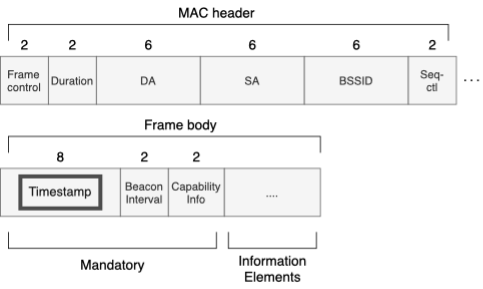
\includegraphics[scale=0.5]{Beacon.drawio.png}
\caption{The beacon frame structure containing the timestamp.}
\label{fig:tsf}
\end{figure}

Besides beacon frames, AP has the responsibility to send a probe response frame when receiving a probe request frame from STAs. And the timestamp field also presents in the probe response frame. No matter whether the frame we’re going to send is a beacon or probe response, we need to explicitly insert TSFT in the timestamp field in the frame body.

The following is the code for getting the TSFT and inserting it into the frame:

\begin{lstlisting}
tsf = wtap_hal_get_tsf(sc->hal);
wh = mtod(m, struct ieee80211_frame *);
memcpy(&wh[1], &tsf, sizeof(tsf));
\end{lstlisting}

First, we get TSFT from wtap HAL, then use the \lstinline{mtod} macro to get the starting address of the frame structure in \lstinline{mbuf}. Finally, we copy the TSFT to the timestamp field which is pointed by \lstinline{&wh[1]}, thus the frame contains the information of TSFT, and is ready to be sent.

\subsubsection{Beacon generation and TSF in IBSS mode}
In IBSS mode, beacon generation is slightly different from infrastructure mode. The beacon frame is only sent by the “oldest” STA in an IBSS, and the “oldest” STA is the one that has the largest TSFT.

\subsubsection{IBSS merge}
IBSS merge is needed to support IBSS mode in every net80211(4) drivers. The term and operations of IBSS merge comes from Wi-Fi Alliance and are adopted by net80211(4).

Before telling the mechanism of the IBSS merge, we have to introduce the unexpected situation which happens without the IBSS merge. Let's begin by creating two IBSS STA with the same SSID "test", and bring up both of them. 

\begin{lstlisting}
wlan0: flags=8843<...> mtu 1500
       ether 00:98:9a:98:96:97
       groups: wlan
       ssid test 
       channel 1 (2412 MHz 11b) 
       bssid b6:e8:81:86:f8:9c
       ...
wlan1: flags=8843<...> mtu 1500
       ether 00:98:9a:98:96:98
       groups: wlan
       ssid test 
       channel 1 (2412 MHz 11b) 
       bssid 12:a3:44:24:c7:61
       ...
\end{lstlisting}

As you can see, both of them have different randomized BSSIDs. In IBSS mode, BSSID is not the same as the STA's mac address, instead, BSSIDs are created by the random-number generator.

After an adequate amount of time, we can start the ping(8) test between the two IBSS STA. The wireless environment of the ping(8) test is shown in the figure \ref{fig:IBSS-mac}.

\begin{figure}[h]
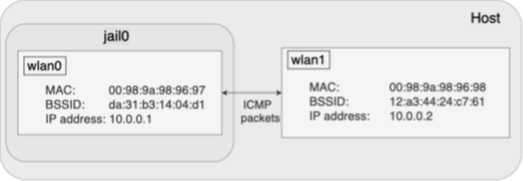
\includegraphics[scale=0.4]{ping-mac-horizontal-modified.png}
\caption{Testing environment of wtap in IBSS mode}
\label{fig:IBSS-mac}
\end{figure}

And Unfortunately, the ping(8) test will fail:

\begin{lstlisting}
$ sudo jexec jail0 ping -c 2 10.0.0.2
PING 10.0.0.2 (10.0.0.2): 
56 data bytes
ping: sendto: Host is down
ping: sendto: Host is down

--- 10.0.0.2 ping statistics ---
2 packets transmitted, 0 packets 
received, 
100.0% packet loss
\end{lstlisting}

The following is the debug message in dmesg(8):

\begin{lstlisting}
wlan1: [da:31:b3:14:04:d1] 
discard frame, 
adhoc_input:407: not to bss
\end{lstlisting}

By tracing \lstinline{adhoc_input()} in \lstinline{src/sys/net80211/ieee80211_adhoc.c}, the reason of the error “not to bss” is that IBSS STA received a frame that has a different BSSID than the STA’s, so net80211 just filtered it out because it thinks the packet is not for the STA.

IBSS merge solves the issue by changing STA's BSSID to match what the “oldest IBSS” has when the SSIDs are the same.

Net80211 has some functions to initiate the IBSS merge, wtap just needs to do some condition check when there is a need to call them.

IBSS merge is issued when receiving a beacon frame or receiving a probe response frame. The following is the step-by-step explanation of the codes for initiating the IBSS merge in \lstinline{vap->iv_recv_mgmt}.

When receiving a management frame, we check whether the frame is a beacon or a probe response. 
\begin{lstlisting}
switch (subtype) {
    case IEEE80211_FC0_SUBTYPE_BEACON:
    case IEEE80211_FC0_SUBTYPE_PROBE_RESP:
\end{lstlisting}

If yes, then do some condition checks:

\begin{lstlisting}
if (vap->iv_opmode == IEEE80211_M_IBSS 
    && vap->iv_state == IEEE80211_S_RUN 
    && ieee80211_ibss_merge_check(ni))
\end{lstlisting}

The \lstinline{vap->iv_opmode == IEEE80211_M_IBSS} and \lstinline{vap->iv_state == IEEE80211_S_RUN} confirms that the vap is running and is an IBSS vap. The \lstinline{ieee80211_ibss_merge_check()} will do some condition and capability checks. 

And most importantly, check the TSFT from the receiving frame. If the TSFT in receiving frame is grater than itself has, then it means the one who sends the beacon frame or probe response frame is the older one in a BSS. So call \lstinline{ieee80211_ibss_merge()} to initiate IBSS merge.

\begin{lstlisting}
uint64_t rx_tsf = ni->ni_tstamp.tsf;
uint64_t self_tsf = 
    wtap_hal_get_tsf(sc->hal);

if (rx_tsf >= self_tsf) {
    (void) ieee80211_ibss_merge(ni);
}
\end{lstlisting}

After the completion of the IBSS merge, the one initiating the IBSS merge will have the same BSSID as the older BSS it merges with.

\subsection{802.11 Frame Capture}
\subsubsection{Radiotap}
Radiotap is a facility designed for capturing 802.11 traffic, including information that is not part of the normal 802.11 frame structure. It’s very useful to have radiotap when debugging the driver.

We have extended the support of radiotap in wtap(4), now one can retrieve radio information of wtap(4) vap via tcpdump(8).

Figure \ref{fig:radiotap} shows the radiotap header and its following information (for brief, called radio information) capturing from the transmission of a probe request frame.

\begin{figure}[H]
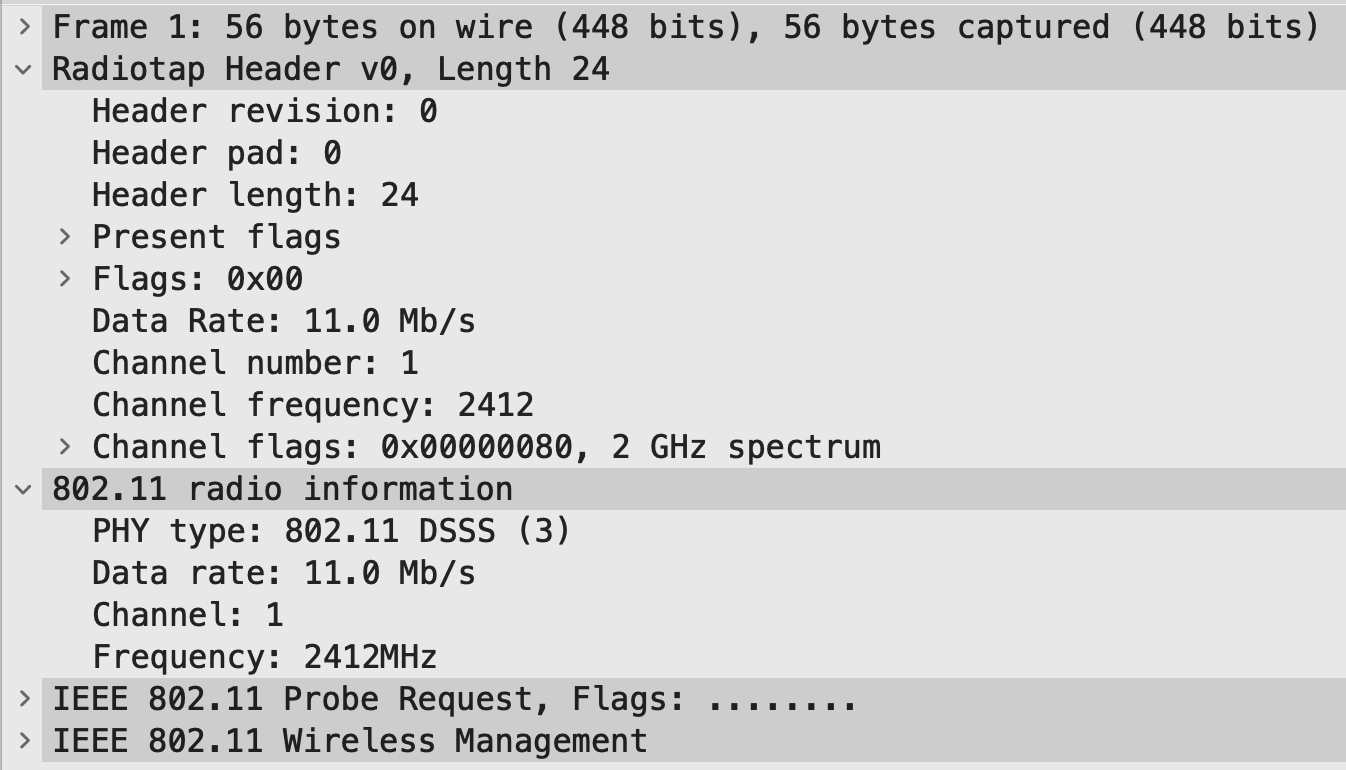
\includegraphics[scale=0.17]{radiotap-tx-modified.png}
\caption{Probe request frame containing radiotap header and radio information.}
\label{fig:radiotap}
\end{figure}

As you can see, radiotap contains some information that 802.11 frames lack, like 802.11 PHY type, data rate, and channel attributes. In the RX frame, TSFT is also presented.

To support radiotap, wtap needs to fill in the per-packet capture state when TX/RX. The state includes data rate and channel information when TX and RX, and TSFT only presents when RX. Here shows the code of filling in channel information into radio information:

\begin{lstlisting}
    th->wt_chan_flags = 
        IEEE80211_CHAN_2GHZ;
    th->wt_chan_freq = 
        ic->ic_curchan->ic_freq;
    th->wt_chan_ieee = 
        ic->ic_curchan->ic_ieee;
    th->wt_chan_maxpow = 0;
\end{lstlisting}

We respectively assign channel flags, channel frequency, channel IEEE (channel number specified in IEEE 802.11 2007 \cite{IEEE80211_2007}), and the maximum power of the channel.

Radiotap only presents when one or more than one process is capturing packets on a vap via tools like tcpdump(8). Remember that the radiotap is for capturing extended information, so it's useless to have the radiotap when no one is capturing it. 

So the TX path is like this: first, verify whether someone is capturing this vap via \lstinline{ieee80211_radiotap_active_vap()}, if yes, then fill in the radio information by the method mentioned earlier, and pass the frame (precisely, entire mbuf) and radio information to bpf(4) via \lstinline{ieee80211_radiotap_tx()}:

\begin{lstlisting}
if (
ieee80211_radiotap_active_vap(vap)) {
    wtap_tx_tap(sc);
    ieee80211_radiotap_tx(vap, m);
}
\end{lstlisting}

It's a little bit different from the RX path. Before passing the frame up to net80211(4) via \lstinline{ieee80211_input()}, we just need to fill in radio information. There is no need to call \lstinline{ieee80211_radiotap_rx()} since after the frame is passed up to net80211(4), net80211(4) will pass the frame and radio information we just filled into bpf(4) if someone is capturing this vap.

\subsubsection{Monitor Mode}
A monitor mode vap acts like a watcher and passes up all traffic it receives even if the traffic is not for itself (sometimes called promiscuous mode), thus is very useful in debugging. 

Enabling wtap(4) supports monitor mode is simply adding the capability \lstinline{IEEE80211_C_MONITOR} in \lstinline{ic->ic_caps}, since the net80211(4) has already customized the input function \lstinline{monitor_input()} for monitor vap, and other vap callbacks are also modified to fit the needs of monitor mode. 

Every input packet from monitor vap will then be passed to bpf(4) for capturing and will not go to the upper protocol stack.

\section{Experiment}
Testing net80211(4) is the goal for wtap(4). The simplest experiment is to do a ping(8) test between two wtap vap running on the same operating mode. If they both succeed in the transmission and reception of ICMP packets, it means net80211(4) has already successfully handled the packets so the lower-level wtap(4) and upper-level protocol stack can see the packets.

In this chapter, we first describe why we need to isolate the network stacks from every vap, then introduce the user-space tool wtapctl(8), and finally go into the per-operating-mode testing.

We also have written a test script in atf-sh(3) for automatically building and testing wtap(4) and net80211(4). The patch can be found in \cite{commit:atf}.

\subsection{Isolation of Network Stack}
To do the ping(8) test, we need to isolate the network stack (precisely, the routing table) of every vap, otherwise, the network stack will find that the two (or more) vaps are on the same host and lo(4) will be used instead of wtap(4). The isolation of the protocol stack is done by jail(8) and vnet(9).

\subsection{User-space tool wtapctl(8)}
We have introduced the new tool wtapctl(8) for controlling two aspect of wtap(4): device manipulation and visibility control. The wtapctl(8) utility has replaced the older tools located in tools/tools/wtap and is now located in usr.sbin, as it is necessary for building wtap(4).

The wtapctl(8) is introduced in the patch \cite{commit:wtapctl}. 

We will see how wtapctl(8) works with wtap(4) to build the experiment environment in the next section.

\subsection{IBSS Mode}
Figure \ref{fig:ibss-test} shows the testing environment of wtap(4) in IBSS mode:

\begin{figure}[h]
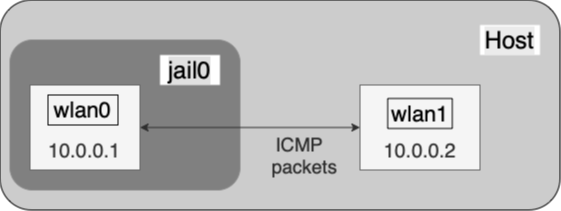
\includegraphics[scale=0.4]{ping-ibss-experiment-modified.png}
\caption{The testing environment of wtap in IBSS mode}
\label{fig:ibss-test}
\end{figure}

Let’s go into more detail.

First of all, we create two wtap devices and enable the traffic between the two devices by the wtapctl(8).

\begin{lstlisting}[caption=Create wtap devices, label={lst:wtap_tool}]
/* Create two wtap devices */
./wtapctl device create // wtap0
./wtapctl device create // wtap1

/* Open wtap medium */
./wtapctl vis open

/* Link two wtap devices */
./wtapctl vis add 0 1
./wtapctl vis add 1 0
\end{lstlisting}

The initial execution of \lstinline{./wtapctl device create} should display \lstinline{wtap0} as the output if it is the first time using wtapctl(8) and no errors occur. Subsequent calls will output \lstinline{wtap1}, and so on. We do not need to assign the unit number since wtap(4) HAL will automatically find the least and not-begin-used number and assign it for us (this is done by the patch \cite{commit:wtapctl}).

We can confirm the creation of wtap devices by wtapctl(8):

\begin{lstlisting}[caption=Show wtap devices, label={lst:sysctl}]
$ wtapctl device list
wtap0 wtap1
\end{lstlisting}

We can now create two IBSS vaps: wlan0 and wlan1, on top of the wtap devices wtap0 and wtap1 respectively, and assign the same SSID "test" for each vap.

\begin{lstlisting}
ifconfig wlan0 create \
wlanmode adhoc wlandev wtap0 \
ssid "test"
ifconfig wlan1 create \
wlanmode adhoc wlandev wtap1 \
ssid "test"
\end{lstlisting}

Before bringing up the two vaps, we suggest that set the debug level of net80211(4) by sysctl(8), to see more details of what's going on to the two vaps in dmesg(8):

\begin{lstlisting}[caption=Debug level, label={lst:debug}]
sysctl net.wlan.0.debug 0xffffffff
sysctl net.wlan.1.debug 0xffffffff
\end{lstlisting}

The debug value of \lstinline{0xffffffff} means all the messages from every IEEE 802.11 debug class will show.

Now it's time to isolate these two vaps. We just need one jail, since putting a vap into the jail and leaving another vap on the host is enough for the isolation of the network stack. We choose to put wlan0 into jail for demonstration.

\begin{lstlisting}[caption=Jail, label={lst:jail}]
jail -c name=jail0 persist vnet \
vnet.interface=wlan0 \
allow.raw_sockets
\end{lstlisting}

Then assign IP addresses to the two vaps. We choose 10.0.0.1 for wlan0 and 10.0.0.2 for wlan1 just for demonstration. At the same time, bring up the two vaps:

\begin{lstlisting}[caption=Assign IP address, label={lst:IP}]
jexec jail0 ifconfig wlan0 \
inet 10.0.0.1/24 up
ifconfig wlan1 inet 10.0.0.2/24 up
\end{lstlisting}

Remember that every IBSS vap will create its IBSS when it is first-time up, hence different BSSIDs for the two vaps. And one of the two vap will do an IBSS merge when it receives a beacon frame or probe response frame that owns the larger TSFT than itself. After that, the two IBSS vap will have the same BSSID and can thus do a ping(8) test.

We can check whether the two vaps have the same BSSID by ifconfig(8). Once we confirm, we can do the ping(8) test. We choose to issue the test on the host, so the target vap will be the one in the jail which owns an IP address of \lstinline{10.0.0.1}.

\begin{lstlisting}[caption=Ping(8) test, label={lst:ping}]
ping -c 5 10.0.0.1
\end{lstlisting}

\subsection{STA/HostAP Mode}
The testing environment is much the same as in IBSS mode shown in Figure \ref{fig:ibss-test}, but this time wlan0 and wlan1 are in HostAP and STA mode respectively.

The building steps of wtap devices is the same as in Listing \ref{lst:wtap_tool}.

Then we can create two vaps: wlan0 (on top of wtap0) for HostAP mode and wlan1 (on top of wtap1) for STA mode. At the same time, assign the same SSID for each of them (assign SSID to STA vap is for future association).

\begin{lstlisting}
ifconfig wlan0 create \
wlanmode hostap wlandev wtap0 \
ssid "test"
ifconfig wlan1 create \
wlanmode sta wlandev wtap1 \
ssid "test"
\end{lstlisting}

Then setting the debug level for each vap in the same way as Listing \ref{lst:debug}, put wlan0 into jail in the same way as Listing \ref{lst:jail}, and assign IP addresses and bring up both of them in the same way as Listing \ref{lst:IP}.

Until now, we still can not do a ping(8) test on these two vaps. It's a bit different in infrastructure BSS from IBSS. An STA vap needs to do authentication and association with the HostAP vap, and only then data frame can be transmitted between the two vaps. 

And unfortunately, we fail to issue the authentication/association request by the user space tool wpa\_supplicant(8). However, the modified ifconfig(8) \cite{commit:mlme} fits the meet. Issuing authentication/association requests via modified ifconfig(8) is shown in the following listing:

\begin{lstlisting}
ifconfig wlan1 assoc 00:98:9a:98:96:97
\end{lstlisting}

The \lstinline{00:98:9a:98:96:97} following the "assoc" is the MAC address of HostAP vap.

We can then confirm whether the STA vap has associated with the HostAP vap by the following commands:

\begin{lstlisting}
ifconfig wlan1 | grep \
"bssid 00:98:9a:98:96:97"
\end{lstlisting}

Finally, the STA vap joins the BSS of the HostAP vap and we can do ping(8) test in the same way as Listing \ref{lst:ping}.

\subsection{Monitor mode}
The testing environment is based on the STA/HostAP mode, plus a monitor vap wlan2 which can hear all traffic between the HostAP vap and STA vap. The following shows the testing environment for monitor mode:

\begin{figure}[H]
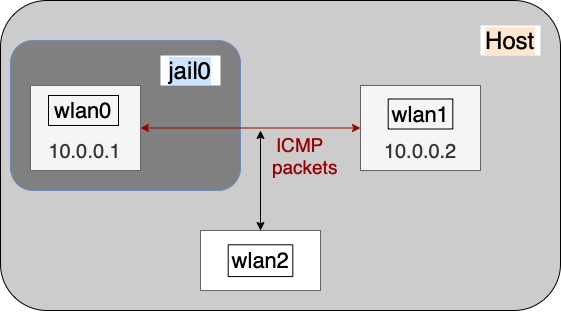
\includegraphics[scale=0.40]{ping_monitor.png}
\caption{Testing environment in Monitor mode.}
\label{fig:monitor}
\end{figure}

As you can see, the monitor vap has no IP address since it's just a layer 2 device and does not pass the receiving packets to the protocol stack. And it also needs not be isolated since it can see all frames on the wtap medium if we set the vis\_map tool correctly.

We took the same way as in STA/HostAP mode building and setting wtap devices, creating a HostAP vap and an STA vap, putting the HostAP vap into jail, assigning IP addresses for HostAP vap STA vap, issuing authentication/association requests on STA vap, except that we have a new Monitor vap. The monitor vap can be built and set by the following steps:

\begin{lstlisting}
/* Create a new wtap device */
./wtapctl device create

/* HostAP device -> Monitor device  */
./wtapctl vis add 0 2
/* STA device -> Monitor device  */
./wtapctl vis add 1 2

/* Create monitor vap */
ifconfig wlan2 create \
wlanmode monitor wlandev wtap2
\end{lstlisting}

From now, all the traffic between HostAP vap and STA vap can be captured by the Monitor vap. We can do a ping(8) test as the same way in Listing \ref{lst:ping}, and capture the ICMP packets by the Monitor vap via tcpdump(8):

\begin{lstlisting}
tcpdump -y IEEE802_11_RADIO -i wlan2
\end{lstlisting}

\section{Conclusion}
Our work has made wtap(4) a more general 802.11 hardware simulator, as we have enhanced it to support additional modes such as IBSS, STA, HostAP, and Monitor, allowing it to be used to test net80211(4) in various operating modes. In addition, we have improved its ability to capture 802.11 frames, making it possible to retrieve TX/RX rate and channel information using tcpdump(8). To facilitate the building and testing process of wtap(4) and net80211(4), we have also developed a test script written in the atf-sh(3) framework (as described in \cite{commit:atf}). To conveniently manipulate the wtap device and visibility plugin, we have introduced the user-space tool wtapctl(8).

In summary, wtap(4) is now a powerful 802.11 simulator that can be used to test net80211(4) without the need for any hardware components. Anyone looking to test or develop net80211(4) should consider using this simulator, and if possible, contribute to expanding its support for more 802.11 features.


\section{References}
\begin{thebibliography}{00}
\bibitem{commit:wtap_origin} https://cgit.freebsd.org/src/commit?id=04d19802897
\bibitem{commit:adhoc} https://cgit.freebsd.org/src/commit?id=c0b65123d09
\bibitem{commit:hostap} https://reviews.freebsd.org/D36243
\bibitem{commit:monitor} https://reviews.freebsd.org/D36469
\bibitem{commit:atf} https://reviews.freebsd.org/D36480
\bibitem{commit:wtapctl} https://reviews.freebsd.org/D37973
\bibitem{IEEE80211_2007} IEEE Std 802.11-2007, 12 June 2007
\bibitem{commit:mlme} https://reviews.freebsd.org/D36242
\end{thebibliography}
\vspace{12pt}

\end{document}
